\documentclass[11pt,a4paper]{scrartcl}

% Setup document
% Import Eidesstattliche Erklärung
\usepackage{pdfpages}
% Import graphics and wrap them
\usepackage{graphicx}
\usepackage{wrapfig}
\usepackage{float}

% Localization
\usepackage[utf8]{inputenc}
\usepackage[T1]{fontenc}
\usepackage[ngerman]{babel}

% Clickable table of contents
\usepackage{hyperref}
\usepackage[ngerman]{cleveref}

% Page formatting
\usepackage[automark]{scrlayer-scrpage}
\usepackage{typearea}
\usepackage{microtype}

% Better tables
\usepackage{tabularray}
\usepackage{booktabs}

% Develop Packages
\usepackage{blindtext}
% Variables
\newcommand{\vorname}{Lukas}
\newcommand{\nachname}{Szimtenings}
\newcommand{\matr}{Matr.-Nr.\ 3217694}
\newcommand{\uni}{FH Aachen}
\newcommand{\studiengang}{Angewandte Mathematik und Informatik}
\newcommand{\modul}{5. Semester 952006 (Aachen)}
\newcommand{\erstpruefer}{Alexander Voß}
\newcommand{\zweitpruefer}{Raphael Majeed}
\newcommand{\subtitel}{ Verteilte Ausführung von in konjunktiver Normalform spezifizierten Machbarkeitsabfragen in medizinischen Datenintegrationszentren }
\newcommand{\titel}{- Seminararbeit -}
\newcommand{\location}{Aachen}
\newcommand{\abteilung}{Abteilung: Research Infrastructure}
\newcommand{\abteilungabkuerzung}{RI}

%images
\newcommand{\uklogo}{
    
\includegraphics[scale=0.5]{res/logo-uniklinik-rwth-aachen}
    
\includegraphics[scale=0.6]{res/imi_sublogo}
}

\newcommand{\ukimilogo}{
\includegraphics[scale=0.16]{res/imilogo}}
% command for wrapfigure -> more than one figure per paragraph
\newcommand*{\invisiblepar}{{\setlength{\parfillskip}{0pt}\par}\vskip-\parskip\noindent\ignorespaces}
% Metadata
\title{\titel}
\author{\vorname{} \nachname}
\date{\today{}, \location}

% Pagestructure
\clearpairofpagestyles
%footer
\ifoot[]{\ukimilogo}
\cfoot[]{\abteilungabkuerzung}
\ofoot[]{\pagemark}
%header
\ihead[]{\vorname\ \nachname}
\chead[]{\titel}
\ohead[]{\matr}
%Seperator
\setheadsepline[\textwidth]{1pt}
\setfootsepline[\textwidth]{1pt}
\addbibresource{Seminararbeit.bib}


\begin{document}
%% Prefix %%
% Titelblatt
\begin{titlepage}
    \centering
    {\scshape\LARGE \uni{} \par \studiengang{} \par \modul{} \par}
    \vspace{1cm}
    {\scshape\Large \titel{} \par}
    \vspace{1.5cm}
    {\bfseries \huge \subtitel{} \par}
    \vspace{2cm}
    {\Large \vorname{} \nachname{} \par \matr{} \par}
    \vfill
    \begin{center}
        \itclogo{}
        \par
        \abteilung{}
    \end{center}

    \par\vfill
    \parbox{4cm}{\hrule \strut{} \centering \footnotesize \vorname{} \nachname{} \par \textit{Autor}}
    \hfill
    \parbox{5cm}{\hrule \strut{} \centering \footnotesize \erstpruefer{} \par \textit{Erstprüfer}}
    \hfill
    \parbox{4cm}{\hrule \strut{} \centering \footnotesize \zweitpruefer{} \par \textit{Zweitprüfer}}
    \vfill
    {\large \location{} \today \par}
\end{titlepage}
% Einbinden der Eidesstattlichen Erklärung
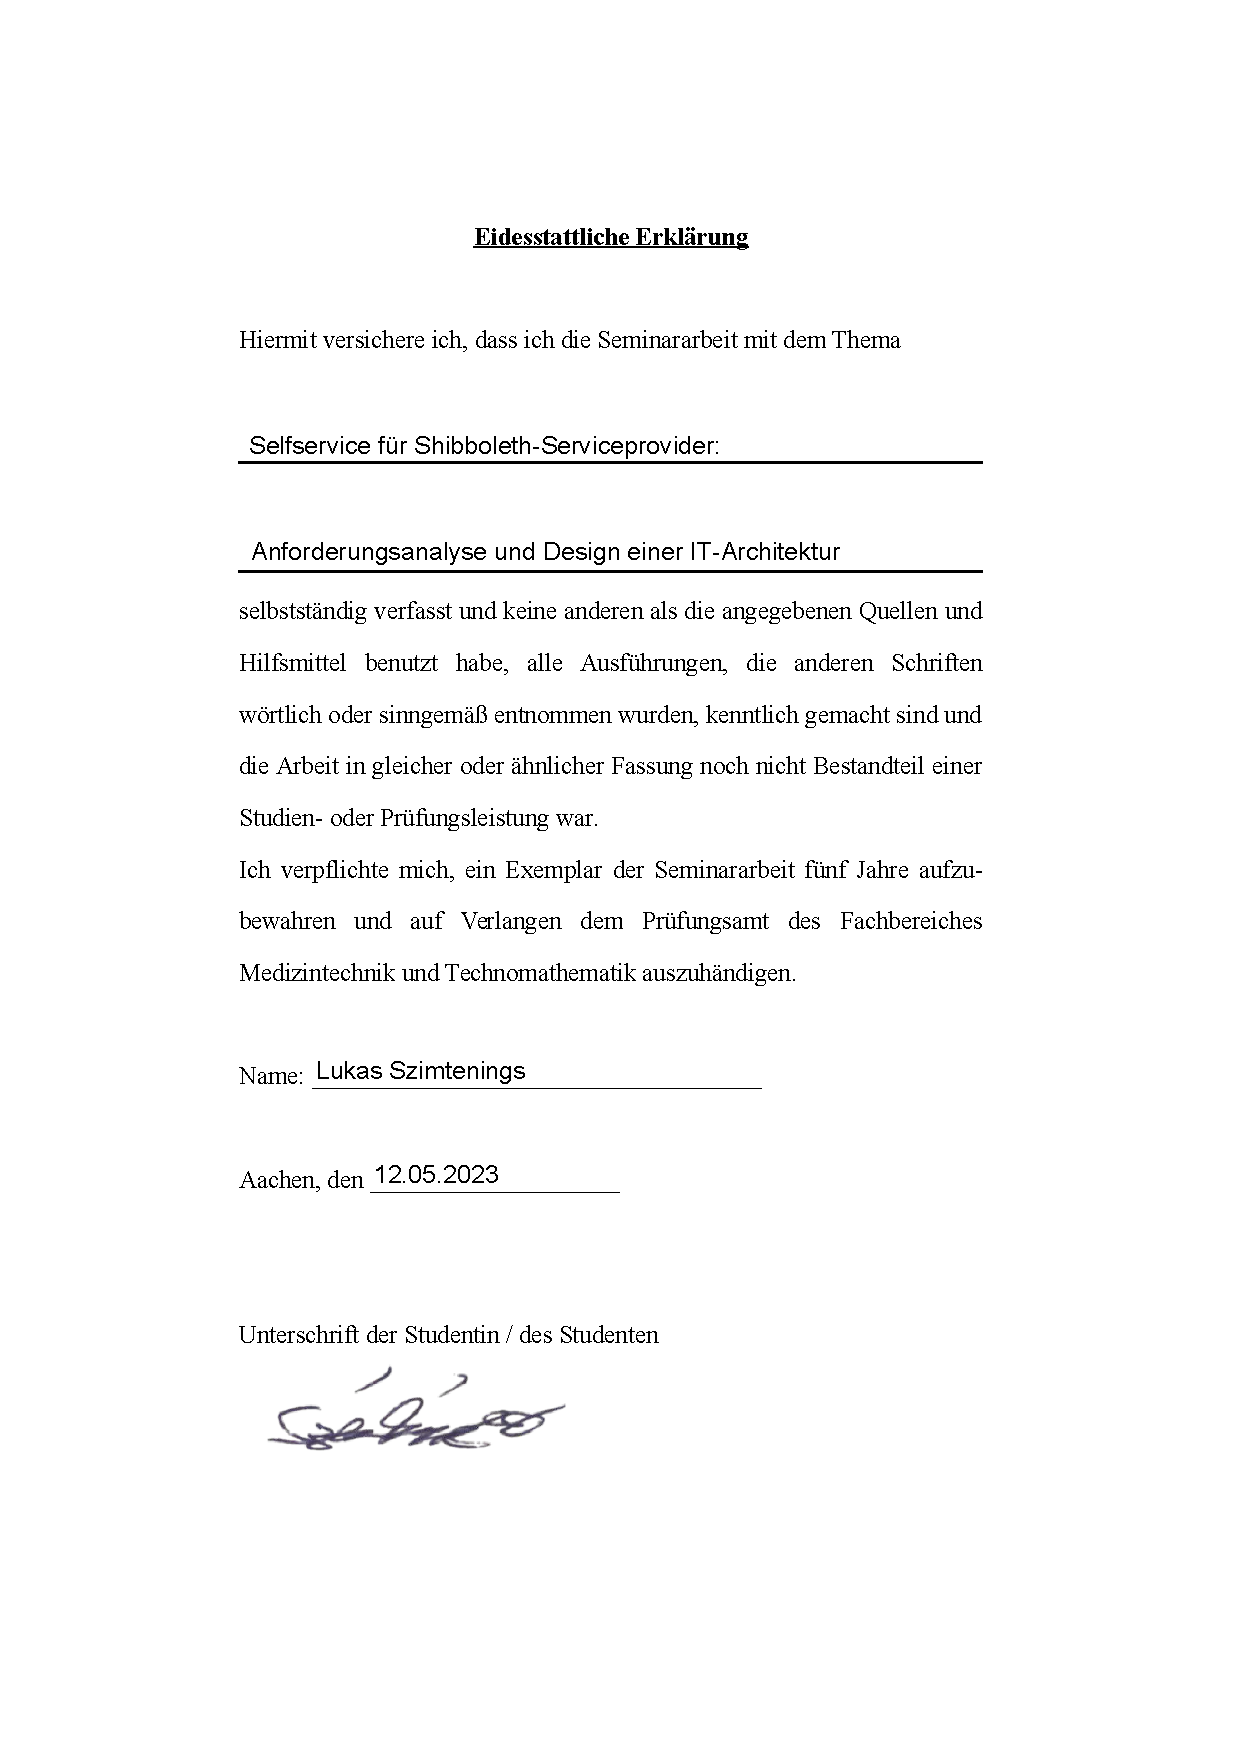
\includepdf{res/EidesstattlicheErklaerung.pdf}
\tableofcontents
\newpage

%% Hauptteil %%
% Seitenzahlen beginnen ab hier
\pagenumbering{arabic}

\section{Einführung}\label{sec:einfuehrung}
Die zunehmende Digitalisierung in Unternehmen führt dazu, dass Prozesse immer mehr automatisiert werden müssen, um wettbewerbsfähig zu bleiben.
Dabei stellt insbesondere die Verwaltung von Zugriffsberechtigungen eine Herausforderung dar, da diese oft sehr komplex und zeitaufwändig ist.
Eine Möglichkeit Zugriffsberechtigungen auf Systeme einer ganzen Organisation und darüber hinweg föderiert zu verwalten ist die Nutzung eines Single Sign-On (SSO) Systems.
Die RWTH Aachen verwendet bereits ein solches System, musste jedoch feststellen, dass durch die Verwaltung von Serviceprovidern ein nicht geringer administrativer Aufwand anfällt.
Zur Entwicklung eines Self-Service Systems muss daher zunächst die Verwaltung von Serviceprovidern auf der Prozessebene analysiert werden.

\subsection{Problemstellung}\label{subsec:problemstellung}
Ein SSO System besteht in aller Regel aus mindestens zwei Komponenten, zum einen dem Identity Provider (IDP) welcher konzeptionell Nutzer authentifiziert und autorisiert, und dem Service Provider (SP) welcher auf Basis der Informationen vom IDP über den Nutzer Zugriff auf seine Ressourcen gewährt.
Das von der RWTH betriebene Shibboleth ist ein solches System, welches vielseitigen Einsatz an der RWTH und übergeordneten Organisationen findet.
Da aus Sicherheitsgründen nicht jeder SP Zugriff auf das SSO System erhalten soll, muss die Verwaltung von SPs zentral in der Hand des IDPs liegen. 
Dies führt jedoch zu einem hohen Verwaltungsaufwand, da die Anzahl der SPs stetig wächst und die Verwaltung der Zugriffsberechtigungen für jeden SP händisch in der IDP Konfiguration erfolgt.
Da die Konfigurationsdatei eine Sicherheitsrelevante Resource darstellt, ist die Anzahl der Personen die diese bearbeiten dürfen begrenzt.

\subsection{Zielsetzung}\label{subsec:zielsetzung}
Ziel dieser Seminararbeit ist es daher, die Verwaltung von SPs auf der Prozessebene zu analysieren und zu modelieren.
In einer Anforderungsanalyse soll dann erarbeitet werden, welche Anforderungen ein Self-Service System erfüllen muss um möglichst viele Teilprozesse an SP Betreiber auszulagern.
\subsection{Abgrenzung}\label{subsec:abgrenzung}
Nicht Ziel dieser Arbeit ist es, ein Systementwurf oder gar Code zu erstellen.
Es soll lediglich eine Analyse der Prozesse erfolgen, und auf Basis dieser eine Anforderungsanalyse durchgeführt werden.


\section{Grundlagen}\label{sec:grundlagen}
   \subsection{Prozessanalyse}\label{subsec:prozessanalyse}
   \subsection{Anforderungsanalyse}\label{subsec:anforderungsanalyse}

\section{Methodik}\label{sec:methodik}
Hier erkläre ich warum ich welche der oben genannten Methoden gewählt habe und wie ich sie im Detail angewandt habe
\subsection{Prozessmodelierung}\label{subsec:prozessmodelierung-methodik}
\subsection{Entwurf des Fragenkatalogs}\label{subsubsec:entwurf-fragenkatalog}
\subsubsection{Auswahl der Gesprächspartner}\label{subsubsec:auswahl-gespraechspartner}

Die Festlegung der Stakeholder-Gruppen für die Befragung zum Zwecke der Prozessmodellierung erfolgte durch eine Dokumentenanalyse der öffentlich zugänglichen Shibboleth-Dokumentation. 
Die Dokumentenanalyse ist eine manuelle Technik zur Business Process Discovery, die im Abschnitt \ref{subsubsec:discovery-manuelle-techniken} kurz vorgestellt wird. 

\subsection{Identity Provider (IDP)}
Die zentrale Rolle der IDPs bei der Verwaltung von Metadaten und der Bereitstellung von Zugriffskontrollen wurde durch die Dokumentenanalyse der Shibboleth-Dokumentation ermittelt. 
Aufgrund ihrer Verantwortung für die Eingabe und Aktualisierung von Metadaten wurde die Stakeholder-Gruppe der IDP-Administratoren ausgewählt.

\subsection{Service Provider (SP)}
Die Dokumentenanalyse der Shibboleth-Dokumentation verdeutlichte desweiteren die Verantwortung der SPs für die Bereitstellung von Diensten und die Umsetzung von Zugriffsrichtlinien, die auf den vom IDP gelieferten claims basieren.
Um den Reibungslosen Ablauf der Kommunikation mit dem IDP sicher zu stellen, müssen die SPs den IDP mit ihren Metadaten versorgen, und diese bei Änderungen aktualisieren.
Die Stakeholder-Gruppe der SP-Administratoren wurde daher ausgewählt, um ihre Erfahrungen und Anforderungen hinsichtlich der Metadatenverwaltung zu untersuchen.

\subsubsection{Fragenkatalog}
In diesem Abschnitt stellen wir Fragen für die verschiedenen Stakeholder-Gruppen auf: Projektverantwortliche, Administratoren der IDP, die für die Eingabe von Metadaten verantwortlich sind, und Serviceanbieter-Administratoren. 
Diese Fragen zielen darauf ab, detaillierte Informationen zur Verwaltung von Metadaten zu sammeln und ihre Relevanz für das Prozessmodellierung zu untersuchen.
Die Erstellung des Fragenkatalogs ist auf Grundlage der in Kapitel~\ref{subsec:interviews-grundlagen} vorgestellten Kriterien erfolgt.

\textbf{Administratoren des IDP}
\begin{enumerate}
    \item \textbf{Frage}: Welche verschiedenen Metadaten werden derzeit verwaltet?
    \item \textbf{Frage}: Wie werden Metadatenänderungen kommuniziert und wie wird sichergestellt, dass alle relevanten Parteien informiert werden?
    \item \textbf{Frage}: Wie werden Metadatenänderungen validiert und wie wird sichergestellt, dass bei der Eintragung keine Fehler auftreten?
    \item \textbf{Frage}: Gibt es Schwierigkeiten bei der Verwaltung von Metadaten, die aufgrund des aktuellen Prozesses auftreten?
    \item \textbf{Frage}: Wie werden Metadatenänderungen in der IDP-Konfiguration vorgenommen?
    \item \textbf{Frage}: Wie viel Zeit wird derzeit für die Verwaltung von Metadaten aufgewendet?
\end{enumerate}

\textbf{Serviceprovider-Administratoren}
\begin{enumerate}
    \item \textbf{Frage}: Was sind die wichtigsten Funktionen, die Sie in einer Self-Service-Lösung zur Verwaltung von Metadaten benötigen würden?
    \item \textbf{Frage}: Gibt es spezielle Anforderungen oder Bedenken in Bezug auf die Sicherheit bei der Verwaltung von Metadaten in einem Self-Service-System?
\end{enumerate}

Diese Fragen behandeln die verschiedenen Aspekte der Metadatenverwaltung und deren Relevanz für das Prozessmodellierung aus der Perspektive der verschiedenen Stakeholder-Gruppen.
\subsection{Anforderungsanalyse}\label{subsec:anforderungsanalyse-methodik}
Weiß noch nicht was hier hin soll, aktuell nur für Symmetrie hier

\section{Ergebnisse und Diskussion}\label{sec:results}
\subsection{Prozessanalyse}\label{subsec:prozessanalyse-results}
\subsubsection{Ergebnisse}\label{subsubsec:prozessanalyse-results}
Ergebnisse bestehend aus zunächst den Fragen und Antworten, und dann dem daraus resultierenden Modell des Prozesses
\subsubsection{Diskussion}\label{subsubsec:prozessanalyse-discussion}
Diskussion der Ergebnisse, eventueller Schwächen im Prozess und Verbesserungsvorschläge
\subsection{Anforderungsanalyse}\label{subsec:anforderungsanalyse-results}
Auflistung der erarbeiteten Anforderungen eingeteilt in funktionale und nicht funktionale Anforderungen
\subsubsection{Funktionale Anforderungen}\label{subsubsec:functional-requirements}
\subsubsection{Nicht-funktionale Anforderungen}\label{subsubsec:non-functional-requirements}
\subsubsection{Diskussion}\label{subsubsec:anforderungsanalyse-discussion}

\section{Zusammenfassung und Ausblick}\label{sec:summary}
\subsection{Zusammenfassung}\label{subsec:summary}
\subsection{Ausblick}\label{subsec:outlook}

%% Suffix %%
\newpage

% Bibliographie
\pagenumbering{Roman}
\printbibliography{}
% Abbildungsverzeichnis
\listoffigures
\end{document}